
\section{Contexto Histórico}

    Um problema de biologia relacionado à maneira com que o sistema nervoso central codifica um impulso muscular foi o que levou Hérault, Jutten e Ans a publicarem o trabalho que é considerado a origem da formulação do problema de BSS (Hérault, Jutten \& Ans, 1985). O trabalho consistia em tentar obter um modelo computacional que se comportasse como o cérebro humano no momento em que este, a partir de apenas um único sinal nervoso, interpreta duas funções importantes: a translação e a velocidade angular do movimento muscular. Pode-se dizer este trabalho teve dois principais resultados. O primeiro foi evidenciar a necessidade da aplicação de EOS ao problema. Isto foi fundamental na concepção dos métodos para resolução do BSS [referência]. O segundo foi a modelagem algébrica dos sistemas de mistura e separação, a matéria-prima do caso BSS/ICA.


    Em 1994, Pierre Comon, utilizando-se dos resultados obtidos por Darmois na década de 1950, formalizou o conceito de ICA e relacionou a independência estatística com o problema da BSS. (Comon, 1994)
    
    
    Jean-François Cardoso e Amari obtiveram, de forma independente, um método de otimização altamente empregado em BSS, denominado de gradiente relativo por Cardoso (Cardoso \& Laheld, 1996) e de gradiente natural por Amari (Amari, 1998). Cardoso também introduziu os conceitos de maximização por verossimilhança no problema de BSS (Cardoso, 1998).
    
    
    O trabalho de Bell e Sejnowski (Bell \& Sejnowski, 1995) popularizou o problema do BSS na comunidade de processamento de sinais devido à sua simplicade de implementação combinada com a capacidade de separar uma quantidade considerável de fontes.
    
    No fim da década de 1990, os trabalhos de Karhunen, Pajunen e Oja  (Karhunen, Pajunen \& Oja, 1998) possibilitaram analisar a ICA como uma extensão não-linear da técnica PCA, já bastante conhecida e difundida na comunidade. Isto fez com que a ICA pudesse ser aplicada em vários estágios referentes à análise de dados. Além disso,  o trabalho de  Hyvärinen introduz o conceito de maximização da não-gaussianidade (Hyvärinen, Karhunen \& Oja, 2001), dando origem a um dos algoritmos mais conhecidos para o problema, o FastICA.
    
    
    Atualmente, uma das principais vertentes de estudo do problema de BSS é considerada a dissociação entre BSS e ICA, que pode ser evidenciada por estudos tais como o do framework TRINICON (Buchner, Aichner \& Kellerman, 2004)
    
\section{Descrição do Problema}

\begin{center}
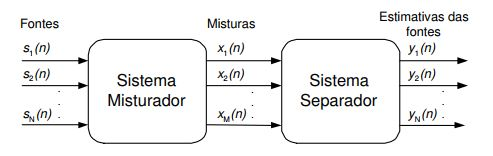
\includegraphics[scale=1.0]{fig221.JPG}
\end{center}


\section{Aplicabilidade}
\subsection{Biomedicina}
\subsection{Telecomunicações}
\subsection{Reconhecimento de voz}
\subsection{Outras aplicações}

\section{Modelagem Matemática do Problema}
% s(n)

$\mathbf{s}$($\mathpzc{n}$) = [$\mathbf{s_1}$($\mathpzc{n}$) $\mathbf{s_2}$($\mathpzc{n}$) \dots  $\mathbf{s_N}$($\mathpzc{n}$)]

% x(n)
$\mathbf{x}$($\mathpzc{n}$) = $\mathcal{F}$($\mathbf{s}$($\mathpzc{n}$), $\mathbf{s}$($\mathpzc{n-1}$), \dots, $\mathbf{s}$($\mathpzc{n - L}$), $\mathbf{n}$($\mathpzc{n}$))

% Linearidade
$\mathcal{F}$($\mathbf{a_1}$$\mathbf{s_1}$($\mathpzc{n}$) + $\mathbf{a_2}$$\mathbf{s_2}$($\mathpzc{n}$)) = $\mathbf{a_1}$$\mathcal{F}$($\mathbf{s_1}$($\mathpzc{n}$)) + $\mathbf{a_2}$$\mathcal{F}$($\mathbf{s_2}$($\mathpzc{n}$))

% Notação Matricial
$\mathbf{x}$ = $\mathbf{A}$$\mathbf{s}$

\section{Análise de Componentes Independentes}
\subsection{Definição}

% Vetor de misturas
$\mathbf{x}$ = [$\mathbf{x_1}$ $\mathbf{x_2}$ \dots  $\mathbf{x_M}$]^T

% Notação Matricial
$\mathbf{y}$ = $\mathbf{W}$$\mathbf{x}$

% Função contraste
$\Phi$($\mathbf{y}$) 

% Permutação
$\Phi$($\mathbf{y}$) = $\Phi$(P . $\mathbf{y}$)

% Escalonamento
$\Phi$($\mathbf{y}$) = $\Phi$($\Lambda$ . $\mathbf{y}$)

% 
$\Phi$($\mathbf{y}$) $\geq$  $\Phi$(A . $\mathbf{y}$)


% vetor de componentes independentes
$\mathbf{y}$ = [$\mathbf{y_1}$ $\mathbf{y_2}$ \dots  $\mathbf{y_N}$]^T

% Probabilidade conjunta independente
$\mathbf{p_{x_1,x_2,\dots,x_N}}$ = $\mathbf{p_{x_1}}$($\mathbf{x_1}$)$\mathbf{p_{x_2}}$($\mathbf{x_2}$)\dots$\mathbf{p_{x_N}}$($\mathbf{x_N}$)

\subsection{Modelo de maximização da não-gaussianidade}
\subsection{Modelo de estimação por máxima verossimilhança}
\subsection{Relação com o problema de BSS}

